\chapter{Aritmética de ideales}

La idea de Richard Dedekind consistía en remplazar las operaciones aritméticas
con elementos $\alpha \in R$ por las operaciones con ideales $I\subseteq R$.
Los anillos de números donde este programa funciona sin obstáculos se conocen
como los \textbf{anillos de Dedekind}. Los vamos a definir en este capítulo.

Una gran parte del material de abajo (ideales primos y maximales, localización,
dominios de valuación discreta, etc.) se encuentra en los libros de texto de
álgebra conmutativa. Recomiendo consultar \cite{Atiyah-Macdonald} y
\cite{Reid-UCA}.

\begin{figure}
  \begin{center}
    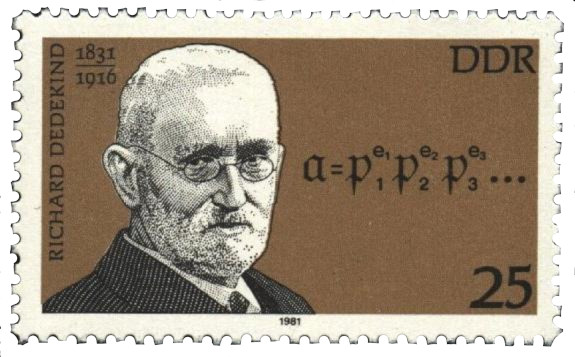
\includegraphics[width=7cm]{pic/Dedekind_stamp.jpg}
  \end{center}

  \caption{Estampilla de la República Democrática Alemana dedicada a Dedekind}
\end{figure}

\pdfbookmark{Clase 5 (24/08/20)}{clase-5}
\section{Operaciones con ideales}
\marginpar{\small Clase 5 \\ 24/08/20}


Sea $R$ un anillo conmutativo. Ya hemos hablado de ideales principales en
el primer capítulo. En general, el ideal generado por elementos
$\alpha_1,\ldots,\alpha_n \in R$ viene dado por
\[ (\alpha_1,\ldots,\alpha_n) =
   \{ c_1 \alpha_1 + \cdots + c_n \alpha_n \mid c_1,\ldots,c_n \in R \}. \]
Los ideales de esta forma se llaman \textbf{finitamente generados}.

\begin{definicion}
  Para los ideales $I, J \subseteq R$ podemos considerar las siguientes
  operaciones.

  \begin{itemize}
  \item La \textbf{suma}
    $$I + J = \{ \alpha + \beta \mid \alpha \in I, \, \beta \in J \}$$
    es el ideal generado por los elementos de $I$ y $J$; en otras palabras,
    el ideal más pequeño que contiene a $I$ e $J$.

    En términos de generadores,
    \[ (\alpha_1,\ldots,\alpha_m) + (\beta_1,\ldots,\beta_n) =
       (\alpha_1,\ldots,\alpha_m,\beta_1,\ldots,\beta_n). \]

  \item El \textbf{producto}
    \[ IJ = \Bigl\{ \sum_{1 \le i \le n} \alpha_i \beta_i \Bigm|
                    n \ge 0, \, \alpha_i \in I, \, \beta_i \in J  \Bigl\} \]
    es el ideal generado por los productos $\alpha\beta$, donde $\alpha \in I$, $\beta \in J$.
    En términos de generadores,
    \[ (\alpha_1,\ldots,\alpha_m) \cdot (\beta_1,\ldots,\beta_n) =
       (\alpha_i \beta_j)_{\substack{1 \le i \le m \\ 1 \le j \le n}}. \]

    Notamos que se cumple $IJ \subseteq I\cap J$.
  \end{itemize}
\end{definicion}

Es fácil verificar que $+$ y $\cdot$ son operaciones asociativas y conmutativas
sobre ideales. Tenemos
$$I + (0) = I, ~ I + R = R, ~ I \cdot (0) = (0), ~ I\cdot R = I.$$
Además, se cumple la distributividad
$$(I + J) H = IH + JH$$
---dejo al lector verificar la doble inclusión.

Ya que hemos definido productos, podemos definir las potencias de la manera
habitual:
\[ I^0 = R, \quad
I^1 = I, \quad
I^2 = I\cdot I, \quad
I^3 = I\cdot I\cdot I, \quad
\ldots \]
Estas nos dan una cadena descendiente
$$R \supseteq I \supseteq I^2 \supseteq I^3 \supseteq \cdots$$

\begin{comentario}
  Cuidado: los elementos de $I^n$ no son productos de $n$ elementos de $I$
  (y mucho menos potencias $\alpha^n$ para $\alpha \in I$), sino \emph{sumas}
  de productos
  $$\sum_{i_1,\ldots,i_n} \alpha_{i_1} \cdots \alpha_{i_n}.$$
  Por ejemplo, en el anillo de polinomios $\ZZ [x]$, consideremos el ideal
  $I = (p,x)$. Entonces $p^2 + x^2 \in I$, pero este elemento no es de la forma
  $fg$ con $f,g \in I$.
\end{comentario}

Notamos que si $J = IH$ para algún $H$, entonces se tiene $J \subseteq H$.
Además, para los ideales principales se cumple
$$\alpha \mid \beta \iff (\alpha) \supseteq (\beta).$$
Esto justifica de alguna manera la siguiente definición.

\begin{definicion}
  Se dice que $I$ divide a $J$ (notación $I \mid J$) si $J \subseteq I$.
\end{definicion}

Sin embargo, hay que tener cuidado: en general no es cierto que $J \subseteq I$
siempre implica que $J = IH$ para algún ideal $H$. Vamos a ver un ejemplo
particular un poco más adelante.

\begin{definicion}
  Se dice que dos ideales $I,J \subseteq R$ son \textbf{coprimos} si
  $I + J = R$.
\end{definicion}

\begin{comentario}
  La motivación detrás del término ``coprimo'' es la siguiente:
  en un dominio de ideales principales (!) se tiene
  \[ (\alpha) + (\beta) = (\alpha,\beta) = (\gamma), \quad
     \text{donde }\gamma = \gcd (\alpha,\beta). \]
  Entonces, $\gcd (\alpha,\beta) = 1$ implica que $(\alpha)+(\beta) = R$.
 
  En general (si $R$ no es un dominio de ideales principales), esto no es
  cierto. Por ejemplo, en el anillo de polinomios $k[x,y]$ se tiene $\gcd (x,y)
  = 1$: los polinomios $x$ e $y$ claramente no tienen divisor en común (excepto
  constantes $c\ne 0$). Por otra parte, $(x,y) \ne k [x,y]$; de hecho,
  $k [x,y]/(x,y) \cong k$.

  Otro ejemplo, más relacionado con lo que estamos estudiando: en el anillo
  $\ZZ [\sqrt{-5}]$ consideremos el ideal $(2, 1 + \sqrt{-5})$. Sus dos
  generadores $2$ y $1 + \sqrt{-5}$ son elementos irreducibles no asociados
  entre sí, y por ende no tienen divisor en común. Sin embargo, no es difícil
  verificar que el ideal en cuestión es propio (y de hecho no es principal).
\end{comentario}

Ahora bien, ¿para qué sirven los ideales y operaciones aritméticas con ellos?
En el capítulo anterior hemos usado en algunas ocasiones que en un dominio
de factorización única, si $\gcd (\alpha,\beta) = 1$
y $\alpha\beta = \gamma^n$, entonces $\alpha$ y $\beta$ (salvo un múltiplo
invertible) son $n$-ésimas potencias: $\alpha \sim \alpha'^n$ y
$\beta \sim \beta'^n$.

Si no hay factorización única, esta propiedad falla.

\begin{ejemplo}
  Ya hemos notado que en el anillo $\ZZ [\sqrt{-5}]$ se tiene
  $$(2 + 3\sqrt{-5})\,(2 - 3\sqrt{-5}) = 7^2,$$
  donde $2 \pm 3\sqrt{-5}$ no es un cuadrado. Para corregir este defecto,
  se puede pasar a los ideales. Pongamos
  \[ I = (2 + 3\sqrt{-5}), \quad J = (2 - 3\sqrt{-5}), \quad H = (7). \]
  Tenemos
  $$I + J = R, \quad I J = H^2.$$
  Ahora
  $$(I + H)^2 = I^2 + I H + H^2 = I\,(I + H + J) = I,$$
  usando que $I + J = R$. De manera simétrica, $(J + H)^2 = J$. Entonces, aunque
  los números $2 \pm 3\sqrt{-5}$ no son cuadrados, los ideales principales
  generados por ellos sí lo son:
  $$(7, 2 \pm 3\sqrt{-5})^2 = (2 \pm 3\sqrt{-5}).$$
  El único detalle es que el ideal $(7, 2 \pm 3\sqrt{-5})$ no es principal;
  de manera contraria, tendríamos $2 \pm 3\sqrt{-5} = \pm\alpha^2$ para algún
  $\alpha$, pero no es el caso.
\end{ejemplo}

El truco de arriba funciona en general.

\begin{proposicion}
  Sean $I, J$ dos ideales tales que $I + J = R$ e $I J = H^n$.
  Entonces, $(I + H)^n = I$.

  \begin{proof}
    Primero una observación: si $I + J = R$, entonces $I^m + J = R$ para todo
    $m$. En efecto,
    \[ R = (I + J)^m =
       I^m + \underbrace{I^{m-1} J + \cdots + I J^{m-1} + J^m}_{\subseteq J}
       \subseteq I^m + J. \]

    Ahora
    \begin{align*}
      (I + H)^n & = I^n + I^{n-1} H + \cdots + I H^{n-1} + H^n \\
                & = I^n + I^{n-1} H + \cdots + I H^{n-1} + I J \\
                & = I\,(I^{n-1} + I^{n-2} H + \cdots + H^{n-1} + J) \\
                & = I,
    \end{align*}
    usando que $I^{n-1} + J = R$.
    \end{proof}
\end{proposicion}

Para terminar con la aritmética básica de ideales, revisemos el teorema chino
del resto. En un dominio de ideales principales este nos dice que
si $\gcd (\alpha,\beta) = 1$, entonces
$$R/(\alpha\beta) \cong R/(\alpha) \times R/(\beta).$$
En un anillo general, hay que considerar ideales coprimos. Primero hagamos
una pequeña observación

\begin{lema}
  Si $I + J = R$, entonces $I \cap J = IJ$.

  \begin{proof}
    Tenemos $IJ \subseteq I\cap J$ en cualquier caso. Ahora si $I + J = R$,
    escribamos $1 = \alpha + \beta$ para $\alpha \in I$, $\beta \in J$.
    Para todo $\gamma \in I \cap J$ se tiene entonces
    $$\gamma = \gamma\,(\alpha + \beta) = \gamma \alpha + \gamma \beta \in IJ.$$
    Esto demuestra la otra inclusión.
  \end{proof}
\end{lema}

Ahora el teorema chino del resto para anillos conmutativos es el siguiente
resultado.

\begin{teorema}[chino del resto]
  Sean $I, J \subseteq R$ ideales tales que $I + J = R$. Luego, hay un
  isomorfismo natural
  \begin{align*}
    R/(IJ) & \xrightarrow{\cong} R/I \times R/J,\\
    \alpha + IJ & \mapsto (\alpha + I, \alpha + J).
  \end{align*}

  \begin{proof}
    Consideremos el homomorfismo
    \[ \phi\colon R \to R/I \times R/J, \quad
       x \mapsto (x+I,x+J). \]
    Vamos a ver que es sobreyectivo y su núcleo es igual a $IJ$.

    Para ver la sobreyectividad, necesitamos probar que para cualesquiera
    $\alpha,\beta\in R$ existe $x\in I$ tal que
    $$x \equiv \alpha \pmod{I}, \quad x \equiv \beta \pmod{J}.$$
    De nuevo, dado que $I + J = R$, escribamos $a + b = 1$ para $a \in I$, $b
    \in J$. Notamos que
    \[ a \equiv 0 \pmod{I}, \quad
       a \equiv 1 \pmod{J}, \quad
       b \equiv 1 \pmod{I}, \quad
       b \equiv 0 \pmod{J}. \]
    Se ve que funcionará el elemento
    $$x = a \alpha + b \beta.$$

    En fin, está claro que $\ker \phi = I \cap J$, y por el lema anterior
    $I \cap J = IJ$.
  \end{proof}
\end{teorema}

\begin{comentario}
  La condición $I + J = R$ es necesaria para la prueba. Por ejemplo, si
  $I = J = 2\ZZ$, entonces $\ZZ/4\ZZ \not\cong \ZZ/2\ZZ \times \ZZ/2\ZZ$.
\end{comentario}

De manera similar, se puede probar que para una familia de ideales
$I_1,\ldots,I_n$ tales que $I_i + I_j = R$ para $i\ne j$, se tiene un isomorfismo
natural
$$R/(I_1\cdots I_n) \cong R/I_1 \times \cdots \times R/I_n$$
(he tomado $n = 2$ en la prueba se arriba solo para simplificar la notación).

\begin{ejemplo}
  Para un primo racional $p \equiv 1 \pmod{4}$ se tiene
  $p = \pi\,\overline{\pi}$ en $\ZZ[i]$. Ya que se trata de un dominio
  de ideales principales, se tiene
  $$(\pi) + (\overline{\pi}) = (\gcd (\pi, \overline{\pi})) = \ZZ[i],$$
  así que por el teorema chino del resto
  \[ \ZZ[i]/(p) \cong \ZZ[i]/(\pi) \times \ZZ[i]/(\overline{\pi})
                \cong \FF_p\times \FF_p. \]
  Otro modo de ver qué está pasando: tenemos
  $$\ZZ[i] \cong \ZZ[x]/(x^2+1), \quad \ZZ[i]/(p) \cong \FF_p [x]/(x^2+1).$$
  Ahora $x^2 + 1$ es irreducible o reducible en $\FF_p [x]$ dependiendo del
  símbolo de Legendre $\legendre{-1}{p} = \pm 1$. Cuando es reducible módulo $p$
  impar, salen dos diferentes factores lineales $x \pm a$, donde $a^2 \equiv -1
  \pmod{p}$.
\end{ejemplo}

%%%%%%%%%%%%%%%%%%%%%%%%%%%%%%%%%%%%%%%%%%%%%%%%%%%%%%%%%%%%%%%%%%%%%%%%%%%%%%%%

\section{Ideales primos y maximales}

El concepto que remplaza la noción de elemento primo es el de \emph{ideal} primo.

\begin{definicion}
  Se dice que un ideal $\mathfrak{p} \subset R$ es \textbf{primo} si este cumple
  una de las siguientes propiedades equivalentes:\footnote{Ejercicio:
    a)$\iff$a${}'$)$\iff$b).}
  \begin{enumerate}
  \item[a)] $\mathfrak{p} \ne R$ y si $\alpha\beta \in \mathfrak{p}$, entonces
    $\alpha \in \mathfrak{p}$ o $\beta \in \mathfrak{p}$;

  \item[a${}'$)] $\mathfrak{p} \ne R$ y si $IJ \subseteq \mathfrak{p}$, entonces
    $I \subseteq \mathfrak{p}$ o $J \subseteq \mathfrak{p}$;
  
  \item[b)] el anillo cociente $R/\mathfrak{p}$ es un dominio.
  \end{enumerate}

  El conjunto de los ideales primos en $R$ se llama el \textbf{espectro}
  de $R$ y se denota por
  $$\Spec R = \{ \mathfrak{p} \subset R \mid \text{ ideal primo} \}.$$

  Se dice que un ideal $\mathfrak{m} \subset R$ es \textbf{maximal} si este
  cumple una de las siguientes propiedades equivalentes:\footnote{Ejercicio:
    a)$\iff$b).}
  \begin{enumerate}
  \item[a)] $\mathfrak{m} \ne R$ y si $\mathfrak{m} \subseteq I \subseteq R$,
    entonces $I = \mathfrak{m}$ o $I = R$;

  \item[b)] el anillo cociente $R/\mathfrak{m}$ es un campo.
  \end{enumerate}
\end{definicion}
(Por la definición, el anillo nulo $R = 0$ no se considera como un dominio,
mucho menos como un campo.)

\begin{proposicion}
  Todo ideal maximal es primo.

  \begin{proof}
    Está claro de la caracterización b).
  \end{proof}
\end{proposicion}

\begin{ejemplo}
  Si $R$ es un dominio de ideales principales, entonces los ideales primos son
  $$\Spec R = \{ (0) \} \cup \{ (\pi) \mid \pi \in R \text{ es primo} \}.$$
  Los ideales de la forma $(\pi)$ son maximales, dado que $R/(\pi)$ es un campo.

  Para verlo, notamos que el ideal principal $(\pi) \subset R$ es primo si y
  solamente si $\pi \in R$ es un elemento primo en el sentido del capítulo
  anterior. En particular,
  \[ \Spec \ZZ = \{ (0) \} \cup \{ (2), (3), (5), (7), (11), \ldots \}. \qedhere \]
\end{ejemplo}

\begin{ejemplo}
  En el anillo $\ZZ [\sqrt{-5}]$ consideremos los ideales
  \[ \mathfrak{p} = (7, 3 + \sqrt{-5}), \quad
     \overline{\mathfrak{p}} = (7, 3 - \sqrt{-5}). \]

  Los ideales en cuestión no son principales: primero, analizando las normas se
  ve que $7$ y $3 \pm \sqrt{-5}$ son elementos irreducibles no asociados
  (las unidades son $\pm 1$). Luego, si $\mathfrak{p} = (\gamma)$, podemos
  considerar las expresiones
  $$7 = \alpha\gamma, \quad 3 + \sqrt{-5} = \beta\gamma$$
  para llegar a una contradicción. Dejo al lector los detalles.

  Estos ideales son coprimos:
  \[ 1 = 7 - (3 + \sqrt{-5}) - (3 - \sqrt{-5})
     \in \mathfrak{p} + \overline{\mathfrak{p}}. \]
  Su producto viene dado por
  \begin{align*}
    \mathfrak{p}\overline{\mathfrak{p}} & = (7, 3+\sqrt{-5})\,(7, 3-\sqrt{-5}) \\
    & = \Bigl(7^2, 7\,(3 + \sqrt{-5}), 7\,(3 - \sqrt{-5}), 14\Bigr) \\
    & = (7)\,(\underbrace{7, 3 + \sqrt{-5}, 3 - \sqrt{-5}, 2}_{= R}) = (7).
  \end{align*}

  Los ideales $\mathfrak{p}$ y $\overline{\mathfrak{p}}$ son propios.
  Por ejemplo, si $\mathfrak{p} = \ZZ [\sqrt{-5}]$, entonces
  para algunos $a,b,c,d \in \ZZ$ se tiene
  \[ 1 = (a + b\sqrt{-5})\cdot 7 + (c + d\sqrt{-5})\cdot (3 + \sqrt{-5})
       = (7a + 3c + 3d) + (7b + c + d)\sqrt{-5}. \]
  De la ecuación $7b + c + d = 0$ podemos expresar $d = -7b-c$,
  y luego al sustituirlo en $1 = 7a + 3c + 3d$ nos queda
  $1 = 7a - 21b$, pero el número a la derecha es par.

  Otra manera más lista es notar que el grupo
  $$\Gal (\QQ (\sqrt{-5})/\QQ) = \{ 1, \sigma \},$$
  donde $\sigma\colon \sqrt{-5} \mapsto -\sqrt{-5}$, actúa sobre
  $\ZZ [\sqrt{-5}]$. Para un ideal $I \subset \ZZ [\sqrt{-5}]$
  el conjunto $\sigma (I)$ es también un ideal, y además, en términos
  de generadores,
  \[ \sigma (\alpha_1,\ldots,\alpha_n) =
     (\sigma (\alpha_1), \ldots, \sigma (\alpha_n)). \]

  En nuestro caso particular se tiene
  $\overline{\mathfrak{p}} = \sigma (\mathfrak{p})$. Ahora si
  $\mathfrak{p} = \ZZ [\sqrt{-5}]$, entonces también
  $\overline{\mathfrak{p}} = \ZZ [\sqrt{-5}]$, pero en este caso
  $\mathfrak{p}\,\overline{\mathfrak{p}} = \ZZ [\sqrt{-5}]$, lo que
  contradice nuestro cálculo de arriba.

  Los ideales $\mathfrak{p}$ y $\overline{\mathfrak{p}}$ son maximales.
  Para verlo, podemos considerar el homomorfismo sobreyectivo
  \[ \phi\colon \ZZ[\sqrt{-5}] \to \FF_7 [x]/(3 + x), \quad
     a + b\sqrt{-5} \mapsto a + b\overline{x}. \]
  (Note que $3^2 \equiv -5 \pmod{7}$.)
  Tenemos $\ker\phi = \mathfrak{p}$, y este ideal es maximal.
  De manera similar se define un homomorfismo sobreyectivo
  $$\overline{\phi}\colon \ZZ[\sqrt{-5}] \to \FF_7 [x]/(3 - x),$$
  donde $\ker\overline{\phi} = \overline{\mathfrak{p}}$.

  Notamos que en general, un homomorfismo $\phi\colon \ZZ [\sqrt{-5}] \to \FF_7$
  está definido por la imagen de $\sqrt{-5}$ que debe cumplir
  $\phi (\sqrt{-5})^2 = -5$ en $\FF_p$. Las únicas posibilidades son
  $\phi (\sqrt{-5}) = \pm 3$, así que hemos encontrado los únicos dos ideales
  maximales que cumplen $\ZZ [\sqrt{-5}]/\mathfrak{p} \cong \FF_7$.

  El teorema chino del resto nos da en este caso
  \[ \begin{tikzcd}
    \ZZ [\sqrt{-5}]/(7) \ar{d}{\cong} &[-3em] \cong &[-3em] \ZZ[\sqrt{-5}]/\mathfrak{p} \ar{d}{\cong} &[-3em] \times &[-3em] \ZZ[\sqrt{-5}]/\overline{\mathfrak{p}} \ar{d}{\cong} \\
    \FF_7 [x]/(x^2 + 5) & \cong & \FF_7 [x]/(3 + x) \ar{d}{\cong} & \times & \FF_7 [x] / (3 - x) \ar{d}{\cong} \\
     && \FF_7 & \times & \FF_7
  \end{tikzcd} \]
\end{ejemplo}

\begin{proposicion}
  Un homomorfismo de anillos $\phi\colon S\to R$ induce una aplicación natural
  entre los espectros
  $$\phi^{-1}\colon \Spec R\to \Spec S, \quad
    \mathfrak{p} \mapsto \phi^{-1} (\mathfrak{p}).$$

  \begin{proof}
    Verifique si $\mathfrak{p} \subset R$ es un ideal primo, entonces
    $\phi^{-1} (\mathfrak{p})$ es un ideal primo en $S$.
  \end{proof}
\end{proposicion}

\begin{ejemplo}
  La inclusión natural $\ZZ \hookrightarrow \ZZ [\sqrt{-5}]$ induce
  una aplicación $\Spec \ZZ [\sqrt{-5}] \to \Spec \ZZ$ dada por
  $\mathfrak{p} \mapsto \mathfrak{p} \cap \ZZ$. En el ejemplo de arriba,
  \[ (7, 3 \pm \sqrt{-5}) \cap \ZZ = 7\ZZ. \qedhere \]
\end{ejemplo}

También nos servirá la siguiente propiedad.

\begin{proposicion}
  Dado un ideal propio $I \subsetneq R$, existe un ideal maximal
  $\mathfrak{m} \subset R$ tal que $I \subseteq \mathfrak{m}$.

  \begin{proof}
    Esta es una aplicación típica del lema de Zorn.

    Sea $\mathcal{P}$ el conjunto de los ideales propios
    $I \subseteq J_\alpha \subsetneq R$ parcialmente ordenado respecto a la
    inclusión $J_\alpha \subseteq J_\beta$. Un elemento maximal en $\mathcal{P}$
    sería precisamente un ideal maximal en $R$ que contiene a $I$. Para deducir
    la existencia de un elemento maximal, tenemos que probar que toda cadena en
    $\mathcal{P}$ es acotada.

    Una cadena en $\mathcal{P}$ es una colección de ideales propios
    $\mathcal{S} = \{ J_\alpha \mid I \subseteq J_\alpha \}$ donde
    $J_\alpha \subseteq J_\beta$ o $J_\beta \subseteq J_\alpha$ para
    cualesquiera $\alpha$ y $\beta$. La unión $J = \bigcup_\alpha J_\alpha$ es
    también un ideal propio en $R$. Este ideal $J$ nos da una cota superior para
    $\mathcal{S}$.
  \end{proof}
\end{proposicion}

Unos de los anillos más fáciles de manejar son anillos locales; más adelante
hablaremos de la localización, pero aquí está la definición de anillos locales.

\begin{definicion}
  Se dice que $R$ es un anillo \textbf{local} si $R$ tiene un único ideal
  maximal $\mathfrak{m}$. En este caso muy a menudo también se escribe
  ``$(R,\mathfrak{m})$ es local''.
\end{definicion}

\begin{ejemplo}
  El anillo
  $\ZZ_{(p)} = \Bigl\{ \frac{a}{b} \in \QQ \Bigm| p\nmid b \Bigr\}$
  es local: su único ideal maximal viene dado por $p\ZZ_{(p)}$.
  De una vez notamos que las unidades son
  $\ZZ_{(p)}^\times = \ZZ_{(p)}\setminus\mathfrak{m} = \Bigl\{ \frac{a}{b} \in \QQ \Bigm| p\nmid ab \Bigr\}$.
\end{ejemplo}

\begin{proposicion}
  Si $(R, \mathfrak{m})$ es un anillo local, entonces
  $R^\times = R\setminus \mathfrak{m}$.

  \begin{proof}
    Si $\alpha \notin R^\times$, entonces el ideal $(\alpha)$ es propio
    y está contenido en $\mathfrak{m}$ que es el único ideal maximal en este
    caso. Viceversa, un elemento $\alpha \in \mathfrak{m}$ no puede ser
    invertible, dado que $\mathfrak{m} \ne R$.
  \end{proof}
\end{proposicion}

Notamos que viceversa, si todos los elementos no-invertibles de $R$ forman un
ideal, entonces este es maximal y $R$ es un anillo local.

%%%%%%%%%%%%%%%%%%%%%%%%%%%%%%%%%%%%%%%%%%%%%%%%%%%%%%%%%%%%%%%%%%%%%%%%%%%%%%%%

\section{Ideales en anillos de números}

Sea $R$ un anillo de números.

\begin{lema}
  Para todo ideal no nulo $I \subseteq R$ se tiene $I \cap \ZZ \ne (0)$.

  \begin{proof}
    Si $\alpha \in I$ es un elemento no nulo, entonces $\alpha$, siendo un
    número algebraico (!), satisface una relación algebraica no trivial
    $$a_n \alpha^n + \cdots + a_1 \alpha + a_0 = 0,$$
    donde $a_i \in \ZZ$, y sin pérdida de generalidad, $a_0 \ne 0$. Entonces,
    $a_0 \in I$.
  \end{proof}
\end{lema}

\begin{corolario}
  Para todo ideal primo no nulo $\mathfrak{p} \subset R$ se tiene
  $\mathfrak{p} \cap \ZZ = p\ZZ$ para algún primo racional $p$.

  \begin{proof}
    La intersección $\mathfrak{p} \cap \ZZ$ debe ser un ideal primo no nulo en
    $\ZZ$.
  \end{proof}
\end{corolario}

\begin{teorema}
  \label{thm:R/I-finito}
  Para todo ideal no nulo $I \subset R$ el cociente $R/I$ es finito.

  \begin{proof}
    Consideremos $R/I$ como un grupo abeliano ($\ZZ$-módulo). Un subgrupo
    finitamente generado de $R/I$ corresponde a un subgrupo finitamente generado
    $M \subseteq R$ tal que $I \subseteq M$.

    Dado que $M \subset K$, donde $K/\QQ$ es un campo de números, $M$ no tiene
    torsión y por ende es un $\ZZ$-módulo libre de rango $r$:
    $$M \cong \underbrace{\ZZ\oplus\cdots\oplus\ZZ}_r.$$
    Notamos que más de $[K : \QQ]$ elementos de $M$ tendrían una dependencia
    $\QQ$-lineal (¡y luego $\ZZ$-lineal!) no trivial.  Esto implica que
    $r \le [K : \QQ]$.

    Denotemos por $M/I$ la imagen de $M$ en el cociente $R/I$.
    Como vimos arriba, $n \in I$ para algún entero $n > 0$, y luego
    $$\# (M/I) \le \# (M/(n)) \le n^{[K : \QQ]}.$$

    Entonces, acabamos de probar que todo subgrupo finitamente generado
    $M/I \subset R/I$ es finito, y además $\# (M/I) \le C$ para cierta constante
    $C$ que no depende de $M$. Esto significa qe $R/I$ es finito.
  \end{proof}
\end{teorema}

\begin{comentario}
  Los argumentos de arriba usan que $R$ es un anillo de números. Sino, podemos
  tomar por ejemplo $R = \ZZ[x]$ y el ideal $\mathfrak{p} = (x)$. Se tiene
  entonces $R/\mathfrak{p} \cong \ZZ$ y $\mathfrak{p} \cap \ZZ = (0)$.

  En este caso $R \subset K$, donde $K = \QQ (x)$, pero la extensión $K/\QQ$
  es infinita de grado de trascendencia $1$.
\end{comentario}

\emph{Continuará...}

\pagebreak

\phantomsection

\addcontentsline{toc}{section}{Ejercicios}
\section*{Ejercicios}

\begin{ejercicio}
  Verifique que para los ideales $I, J, H \subseteq R$ se tiene
  $(I+J)\,H = IH + JH$.
\end{ejercicio}

\begin{ejercicio}
  Encuentre los ideales maximales $\mathfrak{p} \subset \ZZ [\sqrt{-5}]$ tales
  que $\ZZ [\sqrt{-5}]/\mathfrak{p} \cong \FF_{23}$. Demuestre que no son
  principales.
\end{ejercicio}

\begin{ejercicio}
  Dé un ejemplo de grupo abeliano $A$ tal que todo subgrupo finitamente generado
  $B \subset A$ es finito, pero el mismo $A$ es infinito.
  ¿Por qué esto no contradice la prueba de \ref{thm:R/I-finito}?
\end{ejercicio}

\begin{ejercicio}
  Consideremos el anillo $R = \ZZ [\sqrt{13}]$. ¿Cuáles de los siguientes
  ideales son maximales?
  $$(2, 1 + \sqrt{13}), \quad (3, 1 + \sqrt{13}), \quad (5, 1 + \sqrt{13}), \quad(7, 1 + \sqrt{13}).$$
\end{ejercicio}

\begin{ejercicio}
  Demuestre que los ideales primos en $\ZZ [x]$ son los siguientes.

  \begin{itemize}
  \item El ideal nulo $(0)$.

  \item Ideales principales $(f)$ para un polinomio irreducible $f \in \ZZ [x]$.

  \item Ideales maximales $\mathfrak{m} = (p,f)$, donde $p$ es un primo racional
    y $f \in \ZZ [x]$ un polinomio irreducible módulo $p$.
  \end{itemize}

  Concluya que $\dim \ZZ [x] = 2$. Describa $\ZZ [x]/\mathfrak{m}$ para los
  ideales maximales.
\end{ejercicio}

\begin{ejercicio}
  Describa $\Spec k [x,y]$ para un campo $k$ y verifique que $\dim k [x,y] = 2$.
\end{ejercicio}
